% filepath: c:\Users\gabri\Documents\Ceub\tcc\sections\concepts.tex
\chapter{Conceitos}

\section{Fundamentos de Aerodinâmica}
A aerodinâmica é o ramo da física que estuda o comportamento do ar em movimento e sua interação com corpos sólidos, como asas e hélices de aeronaves. O entendimento dos fenômenos aerodinâmicos é fundamental para o projeto eficiente de aeronaves, influenciando diretamente o desempenho, a segurança e a eficiência energética \cite{anderson2017fundamentals}.

\begin{itemize}
    \item \textbf{Sustentação (\(L\))}: força perpendicular ao escoamento do ar, gerada pela diferença de pressão entre as superfícies superior e inferior do perfil aerodinâmico. É responsável por manter a aeronave em voo e depende da forma do perfil, do ângulo de ataque e das condições do escoamento \cite{anderson2017fundamentals}.
    \item \textbf{Arrasto (\(D\))}: força paralela e oposta ao movimento da aeronave, resultante da resistência do ar. O arrasto pode ser dividido em arrasto de forma, arrasto de fricção e arrasto induzido, sendo este último predominante em baixas velocidades e altos ângulos de ataque \cite{raymer2018aircraft}.
    \item \textbf{Eficiência aerodinâmica}: expressa pela razão \(C_L/C_D\), onde \(C_L\) é o coeficiente de sustentação e \(C_D\) o coeficiente de arrasto. Perfis com alta eficiência aerodinâmica proporcionam maior alcance e menor consumo de combustível \cite{abbott1959theory}.
\end{itemize}

Os coeficientes \(C_L\) e \(C_D\) são definidos por:
\[
C_L = \frac{L}{\frac{1}{2} \rho V^2 S}
\qquad
C_D = \frac{D}{\frac{1}{2} \rho V^2 S}
\]
onde \(\rho\) é a densidade do ar, \(V\) a velocidade relativa e \(S\) a área de referência.

Perfis de asas e hélices possuem funções distintas: as asas são projetadas para maximizar a sustentação e minimizar o arrasto em diferentes fases do voo (decolagem, cruzeiro), enquanto hélices convertem potência do motor em tração, transferindo energia para o ar e gerando força propulsora \cite{anderson2017fundamentals}. A otimização de asas normalmente considera decolagem e cruzeiro, pois o pouso envolve dispositivos hipersustentadores e condições operacionais específicas, com menor impacto no desempenho global.

As fases do voo — decolagem, cruzeiro e pouso — apresentam requisitos aerodinâmicos distintos. Na decolagem, busca-se máxima sustentação em baixas velocidades; no cruzeiro, prioriza-se eficiência e baixo arrasto; no pouso, a ênfase está na segurança e controle, frequentemente com uso intensivo de flaps e slats \cite{raymer2018aircraft}. Por isso, a otimização do pouso é usualmente excluída em estudos de desempenho global.

\section{Perfis Aerodinâmicos}
Perfis aerodinâmicos são seções transversais de asas ou hélices, cuja geometria determina o comportamento aerodinâmico do componente. Os principais parâmetros geométricos de um perfil são:

\begin{itemize}
    \item \textbf{Corda (\(c\))}: distância linear entre o bordo de ataque e o bordo de fuga do perfil. É a referência para a maioria dos cálculos aerodinâmicos e influencia diretamente a geração de sustentação \cite{anderson2017fundamentals}.
    \item \textbf{Cambagem}: distância máxima entre a linha média do perfil e a corda. Perfis com maior cambagem tendem a gerar mais sustentação, porém com aumento do arrasto, sendo preferidos em asas de decolagem e manobra \cite{abbott1959theory}.
    \item \textbf{Espessura relativa}: razão entre a espessura máxima do perfil e a corda. Perfis mais espessos proporcionam maior resistência estrutural, mas podem aumentar o arrasto em regimes de alta velocidade \cite{anderson2017fundamentals}.
\end{itemize}

\begin{figure}[H]
    \centering
    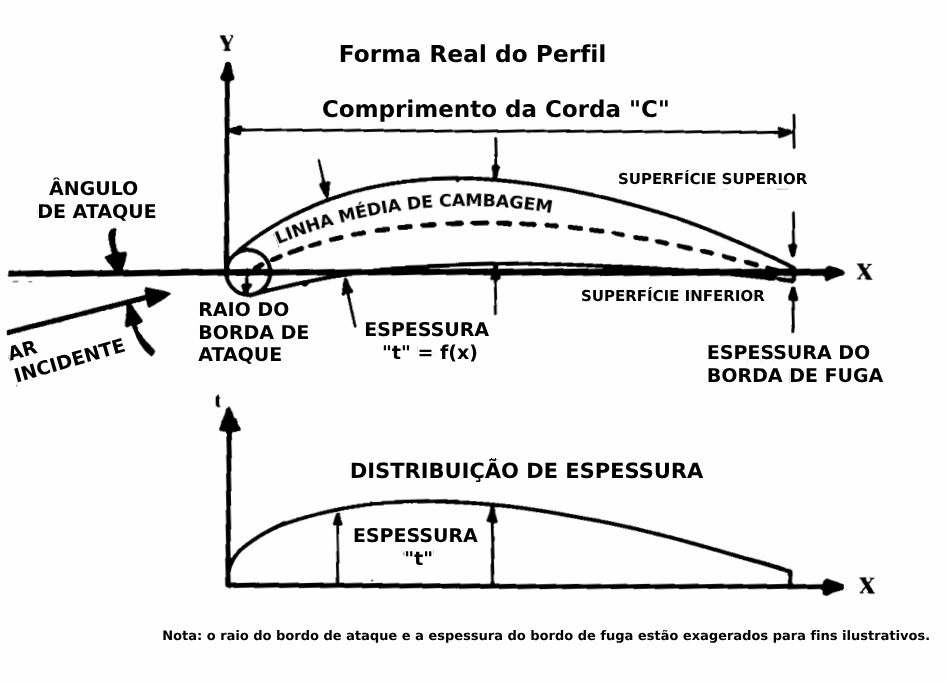
\includegraphics[width=0.6\textwidth]{figuras/perfil_parametros.png}
    \caption{Exemplo de perfil aerodinâmico destacando corda, cambagem e espessura.}
    \label{fig:perfil_parametros}
\end{figure}

A escolha do perfil aerodinâmico é fundamental para o desempenho da aeronave, pois afeta diretamente os coeficientes de sustentação (\(C_L\)) e arrasto (\(C_D\)), além da estabilidade e controle. Perfis simétricos são comuns em hélices e superfícies de controle, enquanto perfis assimétricos (com cambagem) são preferidos em asas para maximizar a sustentação \cite{abbott1959theory}.

Flaps são dispositivos hipersustentadores instalados no bordo de fuga das asas. Quando defletidos, aumentam a curvatura e, consequentemente, a sustentação do perfil, permitindo operações seguras em baixas velocidades, como na decolagem. Durante o cruzeiro, os flaps são recolhidos para minimizar o arrasto e otimizar a eficiência \cite{raymer2018aircraft}.

\begin{figure}[H]
    \centering
    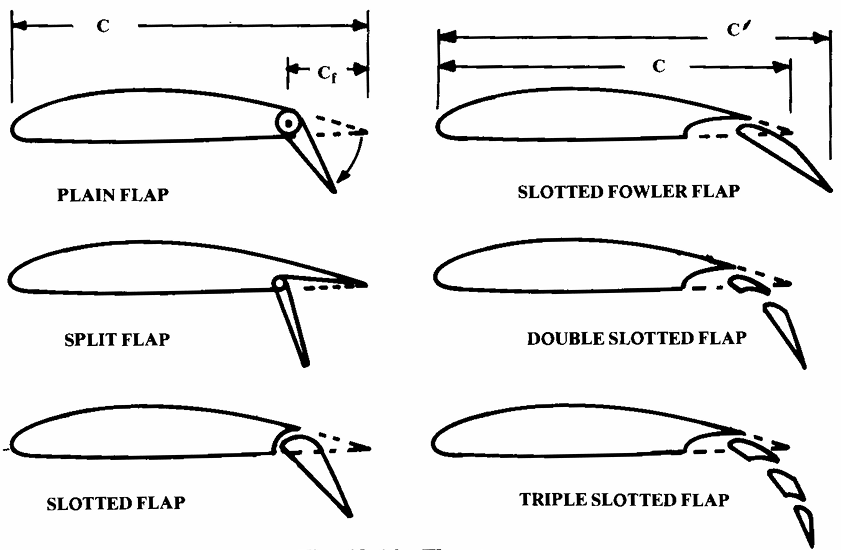
\includegraphics[width=0.6\textwidth]{figuras/perfil_flap.png}
    \caption{Perfil aerodinâmico com e sem flap defletido, ilustrando o aumento da cambagem e da sustentação.}
    \label{fig:perfil_flap}
\end{figure}

A análise detalhada dos perfis aerodinâmicos, incluindo a influência dos flaps e dos parâmetros geométricos, é essencial para a otimização do desempenho em diferentes fases do voo. Estudos clássicos, como os de Abbott e Von Doenhoff \cite{abbott1959theory}, fornecem bases experimentais e teóricas amplamente utilizadas até hoje.

\section{Otimização Computacional}
A otimização computacional em engenharia é um campo multidisciplinar que visa encontrar soluções ótimas para problemas complexos, frequentemente envolvendo múltiplos objetivos e restrições. Os principais métodos aplicados em engenharia aeronáutica incluem:

\begin{itemize}
    \item \textbf{Algoritmos genéticos}: baseados nos princípios da seleção natural, operam sobre populações de soluções, aplicando operadores de cruzamento, mutação e seleção. São eficazes para problemas com múltiplos ótimos locais e espaços de busca extensos \cite{goldberg1989genetic}.
    \item \textbf{Redes neurais}: modelos computacionais inspirados no cérebro humano, capazes de aprender padrões complexos a partir de dados. Em aerodinâmica, são usados para prever coeficientes aerodinâmicos e acelerar processos de otimização \cite{goodfellow2016deep}.
    \item \textbf{Otimização evolutiva}: engloba algoritmos que utilizam mecanismos de evolução, como estratégias evolutivas e programação genética, sendo úteis para problemas de design e ajuste de parâmetros \cite{back1996evolutionary}.
\end{itemize}

O \textit{Xfoil} é uma ferramenta computacional amplamente utilizada para análise de perfis aerodinâmicos, baseada na solução do escoamento potencial e na modelagem da camada limite. Permite calcular coeficientes \(C_L\) e \(C_D\) para diferentes condições de contorno, sendo referência em projetos de asas e hélices \cite{drela1989xfoil}.

\section{Inteligência Artificial em Engenharia}
Inteligência Artificial (IA) refere-se ao desenvolvimento de sistemas capazes de executar tarefas que normalmente requerem inteligência humana, como reconhecimento de padrões, tomada de decisão e aprendizado. Em engenharia, a IA tem sido aplicada para otimização de projetos, análise de dados experimentais, automação de processos e previsão de desempenho \cite{goodfellow2016deep}.

No contexto de otimização aerodinâmica, as principais abordagens de IA são:

\begin{itemize}
    \item \textbf{Redes neurais}: adequadas para modelagem de superfícies de resposta, previsão de coeficientes aerodinâmicos e redução do custo computacional em simulações \cite{goodfellow2016deep}.
    \item \textbf{Algoritmos evolutivos}: eficientes na busca por soluções ótimas em espaços de projeto complexos, especialmente quando o problema apresenta múltiplos objetivos e restrições não lineares \cite{back1996evolutionary}.
\end{itemize}

A escolha entre redes neurais e algoritmos evolutivos depende das características do problema: redes neurais são preferidas para aproximação de funções e análise de grandes volumes de dados, enquanto algoritmos evolutivos são mais indicados para busca global em espaços de soluções complexos \cite{goldberg1989genetic}.